% =============================================================================
% LaTeX Template for Academic Documents
% Author: Nicolas Huber
% Email: nicolas.huber2@uzh.ch
% Github: HuberNicolas
%
% This template is designed for academic and professional documents.
% You are welcome to modify it to suit your requirements. Attribution is appreciated but not mandatory.
% =============================================================================

\documentclass[10pt]{article}

% --- Package Inclusions ---
\usepackage[a4paper]{geometry} % Page layout
 \geometry{
 a4paper,
 total={180mm,257mm},
 left=10mm,
 top=10mm,
 }
\usepackage{amsmath,amssymb,amsfonts} % Mathematical symbols and fonts
\usepackage{zi4} % Font for code listings
\usepackage{graphicx} % Image and figure handling
\usepackage{float} % Enhanced control over float objects
\usepackage{listings} % Code listing support
\usepackage{cite} % Bibliography management
\usepackage{enumitem} % Customized lists
\usepackage{algorithmic} % Algorithm environment
\usepackage{textcomp} % Additional text symbols
\usepackage{xcolor} % Color management
\usepackage{booktabs} % Professional quality tables
\usepackage{hyperref} % Hyperlinks
\usepackage{xparse} % Command parsing
\usepackage{subcaption} % Subfigures and subcaptions
\usepackage{longtable} % Multi-page tables
\usepackage{array} % Enhanced table options
\usepackage{pifont} % Special symbols like ticks and crosses
\usepackage[english]{babel} % Language support
\usepackage{blindtext} % Dummy text
\usepackage{ifthen} % Conditional statements
% --- End of Package Inclusions ---

% --- Custom Commands ---

% ============================ DOCUMENT OPTIONS ===============================

% Highlight a piece of text with a Burnt Orange background
\newcommand{\cmmd}[1]{\colorbox{BurntOrange}{#1}}

% Arrow symbol for inline use
\newcommand{\ar}{$\rightarrow$ }

% Common abbreviations for ease of use
\newcommand{\ie}{\textit{i.e., }} % "that is"
\newcommand{\eg}{\textit{e.g., }} % "for example"
\newcommand{\etal}{\textit{et al. }} % "and others"
\newcommand{\cf}{\textit{cf. }} % "compare with"
\newcommand{\til}{\char`\~} % Tilde symbol

% Custom and specific abbreviations
\NewDocumentCommand{\col}{m}{\textit{#1}}
\newcommand{\gra}{\texttt{Group A }}
\newcommand{\grb}{\texttt{Group B }}
\newcommand{\filename}[1]{\texttt{#1}}


% ============================== HEADER OPTIONS ===============================

% =============================================================================
% University Selection Logic
% =============================================================================
\newcommand{\setuniversity}[1]{%
  \def\universityname{#1}%
  \ifthenelse{\equal{#1}{uts}}{%
    \def\universitylogo{assets/images/uts-logo.png} % UTS logo path
    \def\universitytext{University of Technology Sydney} % UTS name
  }{%
    \def\universitylogo{assets/images/uzh-logo.png} % UZH logo path
    \def\universitytext{University of Zurich} % UZH name
  }%
}

% Set default university if not specified by the user
\setuniversity{uts}

% =============================================================================
% Custom Commands for Title Page Parameters
% =============================================================================

\newcommand{\Course}{Fundamentals of Data Analytics} % Course name
\newcommand{\CourseNo}{30539} % Course number
\newcommand{\Title}{Assessment Task 3: Data Analytics in Action} % Document title
\newcommand{\StudentName}{Nicolas Huber} % Student's full name
\newcommand{\StudentId}{25061944} % Student ID number

% --- End of Custom Commands ---


% --- Custom Colors ---
\definecolor{deepblue}{rgb}{0,0,0.5}
\definecolor{deepred}{rgb}{0.6,0,0}
\definecolor{deepgreen}{rgb}{0,0.5,0}
% --- End of Custom Colors ---

% --- Listing Settings ---
\lstset{
  basicstyle=\ttfamily\scriptsize,
  commentstyle=\color{deepgreen},
  keywordstyle=\color{deepblue},
  stringstyle=\color{deepred},
  showstringspaces=false,
  frame=none, % Options: none, single
  numbers=left,
  numberstyle=\tiny\color{gray},
  breaklines=false,
  postbreak=\mbox{\textcolor{red}{$\hookrightarrow$}\space},
}

\lstdefinestyle{bashstyle}{
  language=bash,
  backgroundcolor=\color{gray!10}, % Light gray background
  morekeywords={dstat, --output},
}

\lstdefinestyle{pythonstyle}{
  language=Python,
  backgroundcolor=\color{gray!10}, % Light gray background
  morekeywords={def, return, if, else, print},
}
% --- End of Listing Settings ---
\begin{document}

\begin{titlepage}
    \centering
    \vspace*{1cm}
    \Huge
    \textbf{\Course}\\
    \vspace{0.5cm}
    \LARGE
    Course Number: \CourseNo\\
    \vspace{1.5cm}
    \textbf{\Title}\\
    \vspace{2cm}
    \textbf{\universitytext}\\
    \vfill
    \includegraphics[width=0.4\textwidth]{\universitylogo}\\
    \vfill
    \Large
    \StudentName\\
    Student ID: \StudentId\\
    Date: \today
\end{titlepage}

\pagenumbering{roman}
\tableofcontents
\newpage

\pagenumbering{arabic}
\section{Introduction}\label{s:introduction}

% \blindtext generates a paragraph of dummy text
\blindtext

\subsection{Generating Multiple Paragraphs}\label{ss:multiple_paragraphs}

% \blindtext[2] generates two paragraphs of dummy text
\blindtext[2]

\subsubsection{Using Blindtext for Filler Content}\label{sss:blindtext_filler}

% The \blindtext command is useful for generating placeholder text in documents.
% It can be used to create a natural flow of content when designing the layout.

\subsection{List Generation Examples}\label{ss:list_examples}

\subsubsection{Itemized Lists}\label{sss:itemized_lists}

% \blinditemize creates a dummy itemize list
\blinditemize

% This subsubsection demonstrates an example of a basic itemized list
% with dummy content using the \blinditemize command.

\subsubsection{Enumerated Lists}\label{sss:enumerated_lists}

% \blindenumerate creates a dummy enumerated list
\blindenumerate

% This subsubsection shows how to generate an enumerated list with dummy content
% using the \blindenumerate command.

\subsubsection{Description Lists}\label{sss:description_lists}

% \blinddescription creates a dummy description list
\blinddescription

% Description lists are often used to associate terms with their definitions or explanations.
% The \blinddescription command generates a placeholder list for such purposes.

\subsection{Mathematical Content}\label{ss:math_content}

% \blindmathpaper generates fake mathematical content
\blindmathpaper

\newpage
\section{Description}\label{s:description}

\newpage
\section{Preprocessing}\label{s:preprocessing}

% Enumerated list
\begin{enumerate}
    \item Dropping non-relevant columns.
    \item Encoding the categorical target variable.
    \item Handling missing values using median imputation.
    \item Scaling numerical features to standardize the data.
    \item Combining all preprocessing steps using \texttt{ColumnTransformer}.
\end{enumerate}

\subsection{Data Encoding and Splitting}
The target variable, \texttt{SpType-ELS}, a categorical variable, was encoded using \texttt{LabelEncoder} to convert categorical values into a binary numerical format. This transformation was essential for compatibility with the machine learning algorithms employed:

% Code example
\begin{verbatim}
label_encoder = LabelEncoder()
y_encoded = label_encoder.fit_transform(y)
\end{verbatim}

% Simple Table
Table \ref{tab:classifiers} summarizes the classifiers used, mapping them to the techniques discussed in class where applicable.
\begin{table}[h!]
    \centering
    \begin{tabular}{lll}
    \hline
    \textbf{Technique}          & \textbf{Concrete Method / Python Function} & \textbf{Week} \\
    \hline
    Decision Tree               & \texttt{DecisionTreeClassifier()}           & Week 7        \\
    Logistic Regression         & \texttt{LogisticRegression()}               & new           \\
    Random Forest               & \texttt{RandomForestClassifier()}            & Week 11       \\
    K-Nearest Neighbors         & \texttt{KNeighborsClassifier()}              & 444           \\
    Support Vector Classifier   & \texttt{SVC()}                               & Week 10       \\
    Multi-layer Perceptron      & \texttt{MLPClassifier()}                     & Week 9        \\
    XGBoost Classifier          & \texttt{XGBClassifier()}                     & new           \\
    Bagging Classifier          & \texttt{BaggingClassifier()}                 & Week 11       \\
    AdaBoost Classifier         & \texttt{AdaBoostClassifier()}                & Week 11       \\
    Gradient Boosting Classifier & \texttt{GradientBoostingClassifier()}        & new           \\
    \hline
    \end{tabular}
    \caption{Mapping of classifiers to discussed techniques in class}
    \label{tab:classifiers}
\end{table}


\subsection{Evaluation Workflow}
The best model and corresponding parameters were determined as follows: Two distinct settings were utilized, corresponding to two independent script executions, with one using 50\% and the other using 100\% of the available training data. The complete pipeline was then run for four different subsets of the data. Each pipeline employed \texttt{GridSearch} to identify the optimal parameters for ten different models. The parameter grid is shown in Table~\ref{tab:hyperparameters}: In total, 124 configurations, an in-depth distribution is depicted in Figure~\ref{fig:grid_search_analysis}, were evaluated using stratified 5-fold cross-validation. For each subset of features, the pipeline identified the best parameters based on model accuracy. The best model was then proposed and evaluated against the test data, with this final evaluation including multiple metrics.


% Complex table
% LaTeX command to adjust row height in tables
\renewcommand{\arraystretch}{1.5} % Adjust this value to increase/decrease row height

% Long table listing
\begin{longtable}[c]{c>{\raggedleft\arraybackslash}p{8cm}}
    \hline
    \textbf{Classifier} & \textbf{Parameter Grid} \\
    \hline
    \endfirsthead
    %
    \multicolumn{2}{c}%
    {{\bfseries Table \thetable\ continued from previous page}} \\
    \hline
    \textbf{Classifier} & \textbf{Parameter Grid} \\
    \hline
    \endhead
    %
    \hline
    \endfoot
    %
    \hline
    \hline
    %\multicolumn{2}{|c|}{End of Table} \\
    %\hline
    \endlastfoot
    %
    Decision Tree Classifier & \begin{tabular}[c]{@{}c@{}} max\_depth: [None, 10, 20, 30],\\ min\_samples\_split: [2, 10, 20],\\ min\_samples\_leaf: [1, 5, 10] \end{tabular} \\
    \hline
    Logistic Regression Classifier & \begin{tabular}[c]{@{}c@{}} C: [0.1, 1.0, 10],\\ solver: [liblinear, lbfgs] \end{tabular} \\
    \hline
    Random Forest Classifier & \begin{tabular}[c]{@{}c@{}} n\_estimators: [200, 300],\\ max\_features: [sqrt, log2] \end{tabular} \\
    \hline
    KNN (K-Nearest Neighbors) & \begin{tabular}[c]{@{}c@{}} n\_neighbors: [1, 3, 5],\\ weights: [uniform, distance] \end{tabular} \\
    \hline
    SVC (Support Vector Classifier) & \begin{tabular}[c]{@{}c@{}} C: [1, 2],\\ kernel: [rbf, sigmoid] \end{tabular} \\
    \hline
    MLPC (Multi-layer Perceptron Classifier) & \begin{tabular}[c]{@{}c@{}} hidden\_layer\_sizes: [(50,), (100,), (50, 50)],\\ activation: [tanh, relu],\\ learning\_rate\_init: [0.01, 0.1] \end{tabular} \\
    \hline
    XGBC (XGBoost Classifier) & \begin{tabular}[c]{@{}c@{}} n\_estimators: [100, 300],\\ max\_depth: [1, 2],\\ learning\_rate: [0.1, 0.3],\\ subsample: [0.7, 1],\\ colsample\_bytree: [0.7, 1] \end{tabular} \\
    \hline
    Bagging Classifier & \begin{tabular}[c]{@{}c@{}} n\_estimators: [10, 50, 100],\\ max\_samples: [0.5, 1.0],\\ max\_features: [0.5, 1.0] \end{tabular} \\
    \hline
    AdaBoost Classifier & \begin{tabular}[c]{@{}c@{}} n\_estimators: [50, 100],\\ learning\_rate: [0.01, 0.1, 1] \end{tabular} \\
    \hline
    Gradient Boosting Classifier & \begin{tabular}[c]{@{}c@{}} n\_estimators: [10, 100],\\ learning\_rate: [0.1, 0.3],\\ max\_depth: [3, 5] \end{tabular} \\
    \caption{Hyperparameters for each model to be tuned during \texttt{GridSearch}}
    \label{tab:hyperparameters}
\end{longtable}

% Figure with 2 subfigures with corresponding captions and one overall caption
\begin{figure}[H]
    \centering
    \begin{subfigure}[b]{0.45\linewidth}
        \centering
        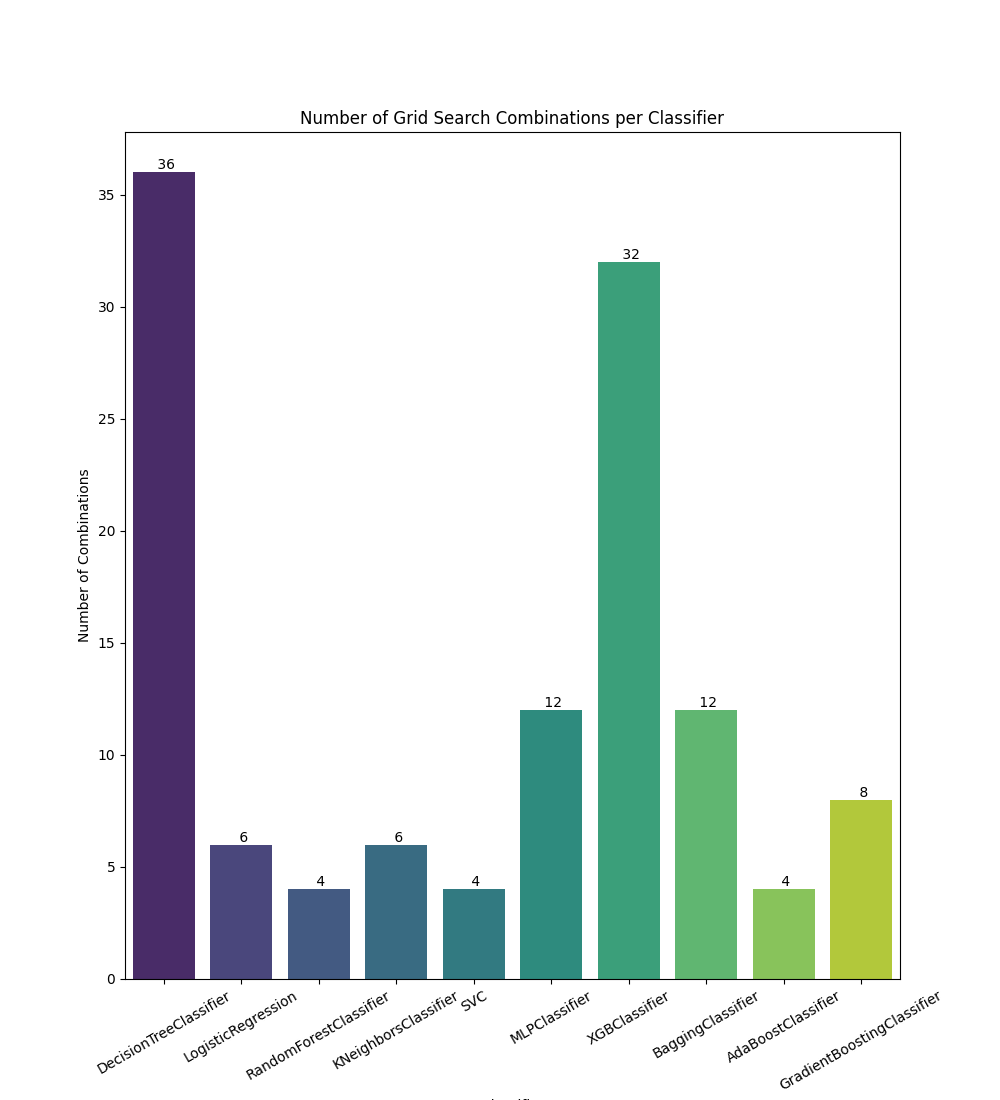
\includegraphics[width=\linewidth]{assets/images/methodology/grid_search_combinations_per_classifier.png}
        \caption{Number of \texttt{GridSearch} Combinations per Classifier (124 in total)}
        \label{fig:grid_search_combinations_per_classifier}
    \end{subfigure}
    \hfill
    \begin{subfigure}[b]{0.45\linewidth}
        \centering
        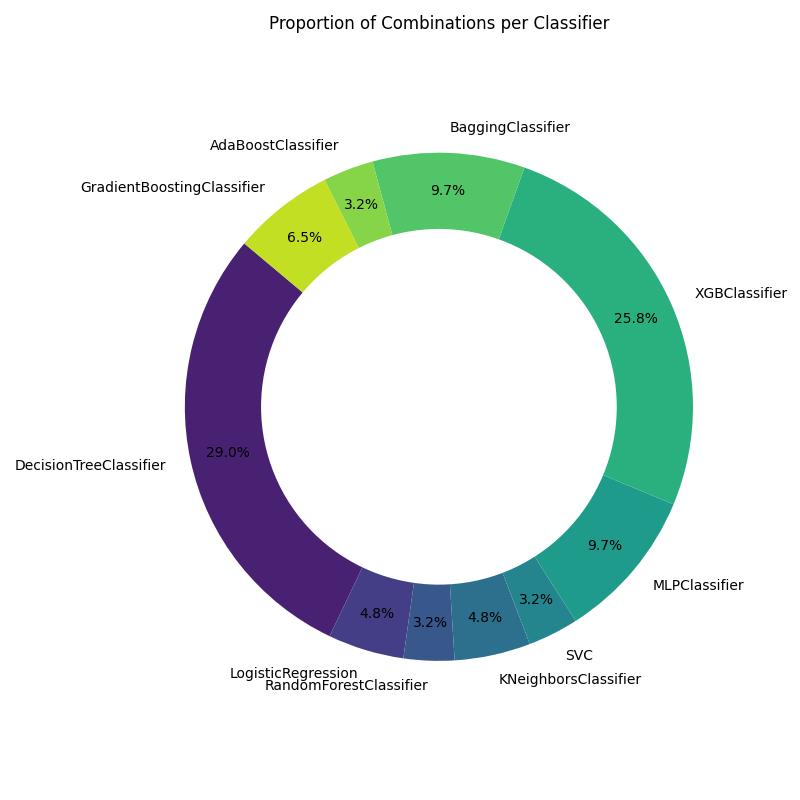
\includegraphics[width=\linewidth]{assets/images/methodology/grid_search_donat.png}
        \caption{Proportion of Combinations per Classifier}
        \label{fig:grid_search_donut}
    \end{subfigure}
    \caption{Analysis of \texttt{GridSearch} Combinations: The left plot shows the number of grid search combinations for each classifier, while the right plot illustrates the proportion of these combinations relative to the total combinations across all classifiers.}
    \label{fig:grid_search_analysis}
\end{figure}

% Full-width figure with one caption
\begin{figure}[H]
    \centering
    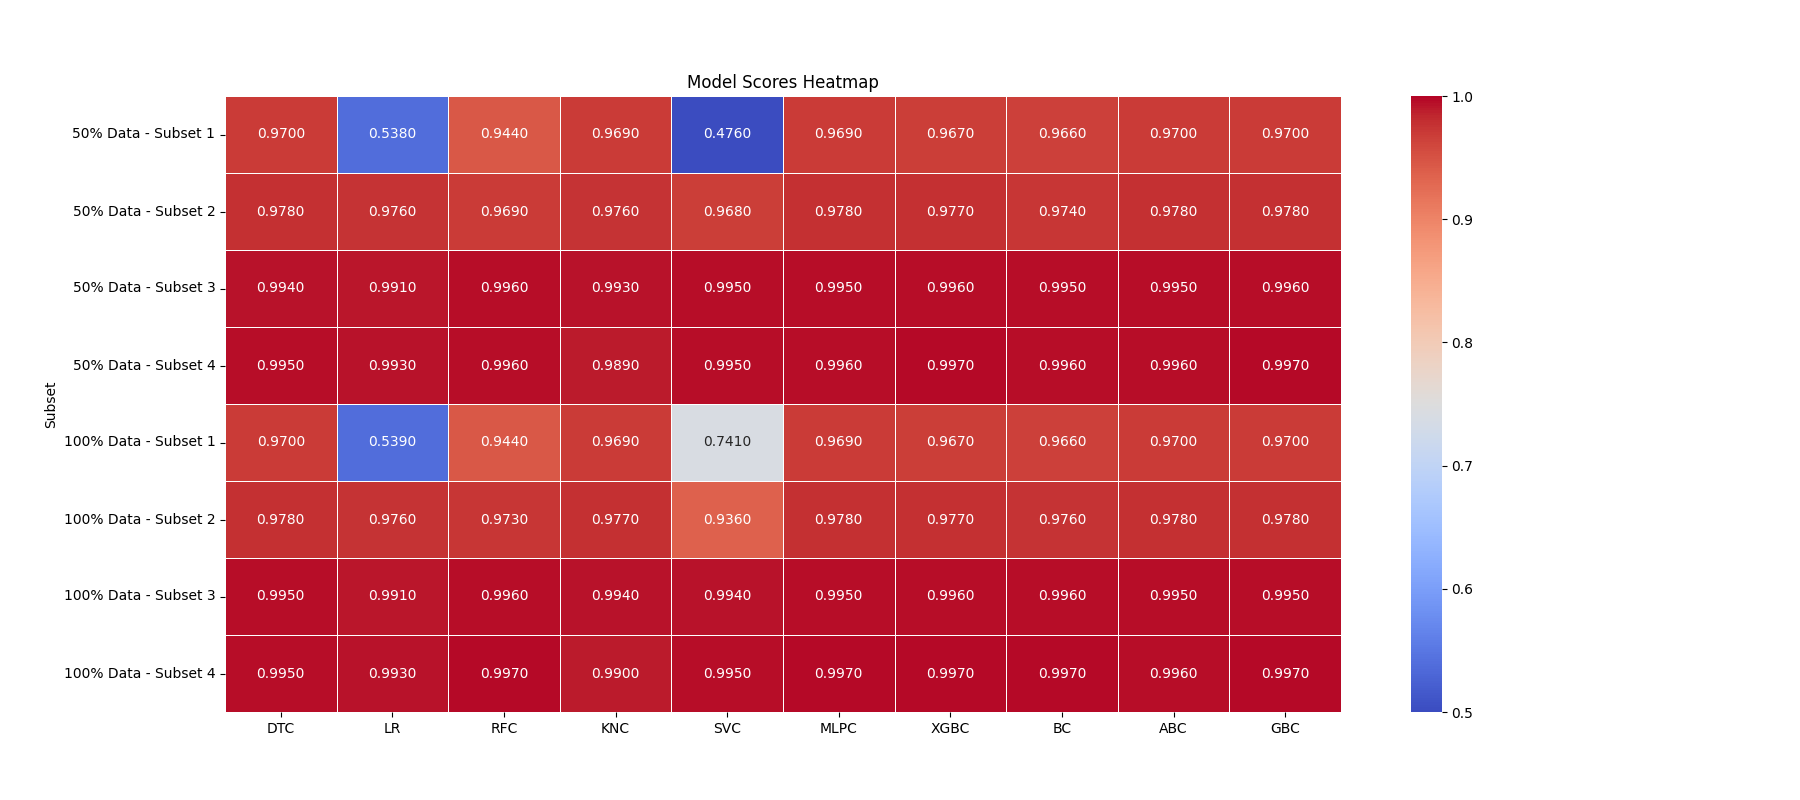
\includegraphics[trim=0cm 0cm 5cm 0cm, clip, width=\linewidth]{assets/images/best_classifier/eval_heatmap.png}
    \caption{Heatmap visualizing the performance of various models with optimal parameters across two different training data sizes (50\% and 100\%) and multiple feature sets. The scores are displayed with increased precision to highlight the subtle differences in model performance. This visualization aids in identifying the most effective models and configurations.}
    \label{fig:eval_heatmap}
\end{figure}

\newpage
\appendix
% Section for the appendix
\section{Appendix}\label{section:appendix}

% Subsection providing a link to the source code repository
\subsection{Source Code}
The interested reader can find the source code \href{https://github.com/HuberNicolas/gaia-classifier}{here}.

\section{Data}

\subsection{Feature Subsets}

% Table including symbolic notation
\begin{table}[h!]
    \centering
    \begin{tabular}{>{\raggedright\arraybackslash}m{3cm}>{\centering\arraybackslash}m{2cm}>{\centering\arraybackslash}m{2cm}>{\centering\arraybackslash}m{3cm}>{\centering\arraybackslash}m{2cm}}
    \hline
    \textbf{Dataset} & \textbf{Size} & \textbf{Accuracy} & \textbf{Symbol} & \textbf{Used} \\
    \hline
    Dataset A & 1000 & 92\% & $\dagger$ & \checkmark \\
    Dataset B & 5000 & 87\% & $x$ & \ding{55} \\
    Dataset C & 2000 & 95\% & $o$ & \checkmark \\
    \hline
    \multicolumn{5}{l}{$\dagger$: Symbol A, $x$: Symbol B, $o$: Symbol C} \\
    \end{tabular}
    \caption{Summary of Datasets and Accuracy}
    \label{tab:datasets}
\end{table}

\section{Evaluation}

% Figure
\begin{figure}[H]
    \centering
    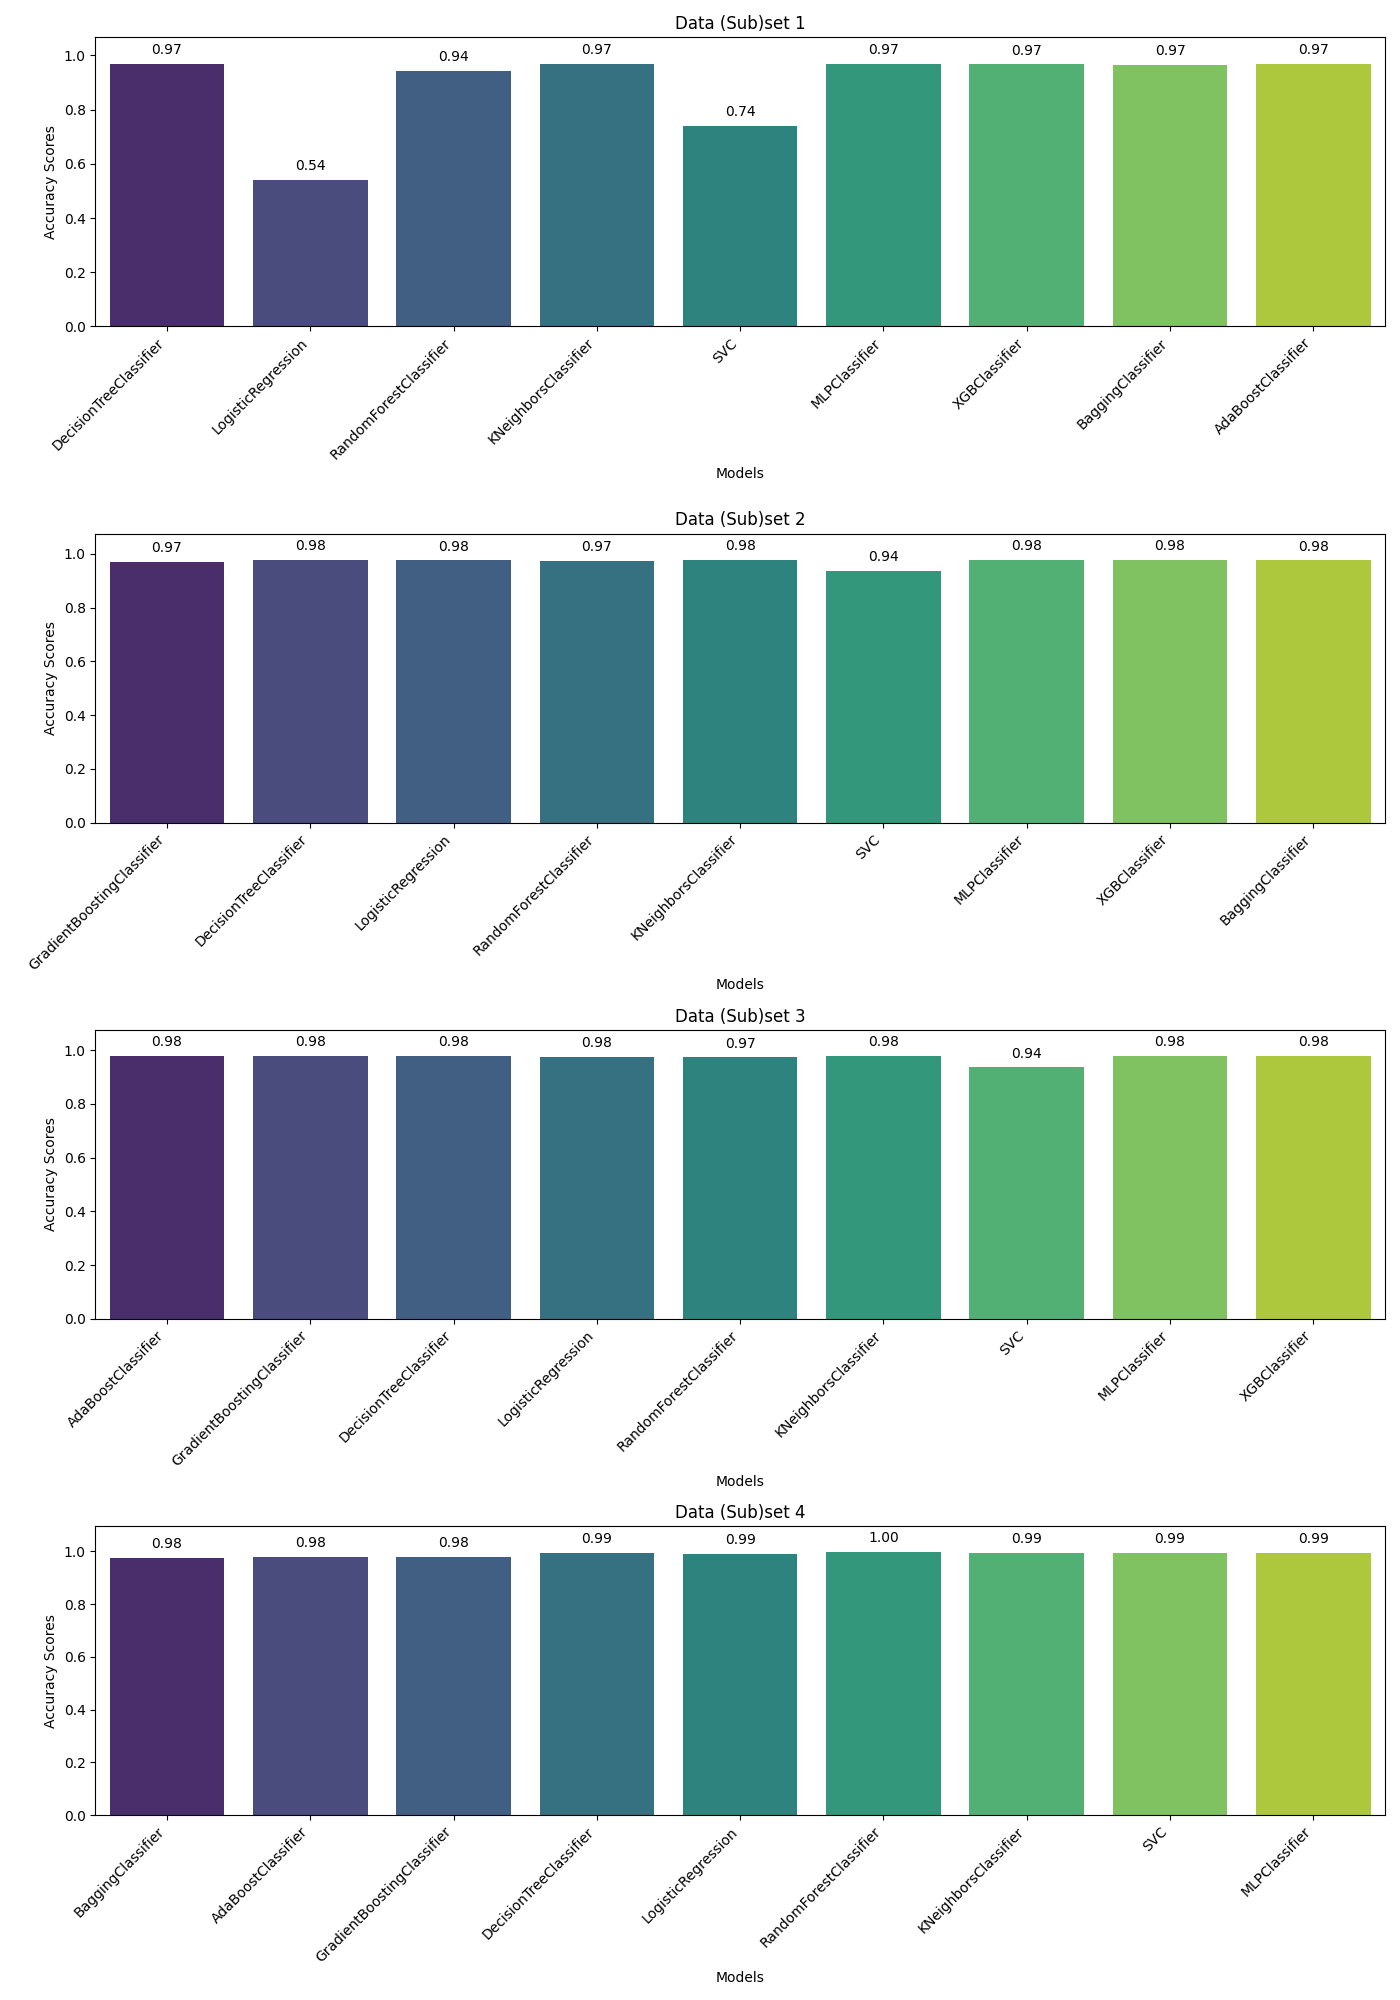
\includegraphics[width=0.8\linewidth]{assets/images/best_classifier/50_data_eval.png}
    \caption{Bar chart illustrating the performance differences of different models on different feature sets (50\% of the training data)}
    \label{fig:eval_bar_scores_50}
\end{figure}

\subsection{In-depth Metrics calculations for the best model}\label{s:calculation}

% Mathematical representation of a confusion matrix used for metric calculations
Based on the following heat map,
\[
\begin{bmatrix}
15950 & 47 \\
35 & 13676 \\
\end{bmatrix}
\]
we evaluate the corresponding scores as follows:

% Inline LaTeX code for calculating various evaluation metrics based on the confusion matrix
\begin{align*}
\text{Accuracy} &= \frac{TP + TN}{TP + TN + FP + FN} = \frac{13676 + 15950}{13676 + 15950 + 47 + 35} = \frac{29626}{29708} \approx 0.9972 \\
\text{Precision} &= \frac{TP}{TP + FP} = \frac{13676}{13676 + 47} = \frac{13676}{13723} \approx 0.9966 \\
\text{Recall} &= \frac{TP}{TP + FN} = \frac{13676}{13676 + 35} = \frac{13676}{13711} \approx 0.9975 \\
\text{Specificity} &= \frac{TN}{TN + FP} = \frac{15950}{15950 + 47} = \frac{15950}{15997} \approx 0.9971 \\
\text{F1 Score} &= 2 \cdot \frac{\text{Precision} \cdot \text{Recall}}{\text{Precision} + \text{Recall}} = 2 \cdot \frac{0.9966 \cdot 0.9975}{0.9966 + 0.9975} \approx 0.9970 \\
\text{False Positive Rate (FPR)} &= \frac{FP}{FP + TN} = \frac{47}{47 + 15950} = \frac{47}{15997} \approx 0.0029 \\
\text{False Negative Rate (FNR)} &= \frac{FN}{FN + TP} = \frac{35}{35 + 13676} = \frac{35}{13711} \approx 0.0026 \\
\text{False Discovery Rate (FDR)} &= \frac{FP}{TP + FP} = \frac{47}{13676 + 47} = \frac{47}{13723} \approx 0.0034 \\
\end{align*}

\newpage
\bibliographystyle{IEEEtran}
\bibliography{references}

\end{document}
